\section{Pregunta N$^{\circ}$1\qquad Andre Gilmer Santos Felix}

\begin{frame}
    \begin{definition}[Polinomio de Bernstein]
        Las funciones base de Bernstein son
        \begin{equation*}
            \forall t\in\left[0,1\right]:
            \forall k\in\left\{0,\dotsc,n\right\}:
            B_{k,n}\left(t\right)\coloneqq
            \binom{n}{k}
            t^{k}
            \left(1-t\right)^{n-k}\in\mathbb{P}_{n}.
        \end{equation*}
        Con la convención
        \begin{math}
            B_{-1,n-1}=
            B_{n,n-1}\equiv0
        \end{math}.
    \end{definition}

    \begin{theorem}
        Se cumple
        \begin{math}
            B^{\prime}_{k,n}\left(t\right)=
            n
            \left(
            B_{k-1,n-1}\left(t\right)-
            B_{k,n-1}\left(t\right)
            \right)
        \end{math}.
    \end{theorem}

    \begin{corollary}
        Se cumple
        \begin{math}
            B^{\prime\prime}_{k,n}\left(t\right)=
            n\left(n-1\right)
            \left(
            B_{k-2,n-2}\left(t\right)-
            2B_{k-1,n-2}\left(t\right)+
            B_{k,n-2}\left(t\right)
            \right)
        \end{math}.
    \end{corollary}

    \begin{proof}
        Sea
        \begin{math}
            B_{k,n}\left(t\right)
        \end{math}
        un polinomio de Bernstein.
        Entonces,
        \begin{align*}
            {\left(
                B^{\prime}_{k,n}\left(t\right)
                \right)}^{\prime}
             & =
            \left(
            n
            \left(
            B_{k-1,n-1}\left(t\right)-
            B_{k,n-1}\left(t\right)
            \right)
            \right)^{\prime}. \\
             & =
            n\left(
            \alert{
                B^{\prime}_{k-1,n-1}\left(t\right)
            }    -
            \alert{
                B^{\prime}_{k,n-1}\left(t\right)
            }
            \right).          \\
             & =
            n\left(
            \alert{
                \left(n-1\right)
                \left(
                B_{k-2,n-2}\left(t\right)-
                B_{k-1,n-2}\left(t\right)
                \right)
            }    -
            \alert{
                \left(n-1\right)
                \left(
                B_{k-1,n-2}\left(t\right)-
                B_{k,n-2}\left(t\right)
                \right)
            }
            \right).          \\
             & =
            n\left(n-1\right)
            \left(
            B_{k-2,n-2}\left(t\right)-
            B_{k-1,n-2}\left(t\right)-
            B_{k-1,n-2}\left(t\right)+
            B_{k,n-2}\left(t\right)
            \right).          \\
             & =
            n\left(n-1\right)
            \left(
            B_{k-2,n-2}\left(t\right)-
            2B_{k-1,n-2}\left(t\right)+
            B_{k,n-2}\left(t\right)
            \right).
        \end{align*}
    \end{proof}
\end{frame}
\begin{frame}
    Sea $\gamma\colon\left[a,b\right]\to\mathbb{R}^{n}$ una curva
    suave.
    \begin{definition}[Longitud de arco]
        La función \alert{longitud de arco} es dada por
        \begin{math}
            \displaystyle
            s\left(t\right)=
            \int\limits_{a}^{t}
            \left\|
            \gamma^{\prime}\left(u\right)
            \right\|\dl u
        \end{math}.
    \end{definition}

    \begin{definition}[Curvatura]
        La \alert{curvatura} es
        \begin{math}
            k\left(t\right)=
            \dfrac{
            \left\|T^{\prime}\left(t\right)\right\|
            }{
            \left\|\gamma^{\prime}\left(t\right)\right\|
            }
        \end{math},
        donde
        \begin{math}
            T\left(t\right)=
            \dfrac{
                \gamma^{\prime}\left(t\right)
            }{
                \left\|\gamma^{\prime}\left(t\right)\right\|
            }
        \end{math}.
    \end{definition}

    \begin{theorem}
        Si $n=3$, entonces
        \begin{math}
            k\left(t\right)=
            \dfrac{
                \left\|\gamma^{\prime}\left(t\right)\times\gamma^{\prime\prime}\left(t\right)\right\|
            }{
                {\left\|\gamma^{\prime}\left(t\right)\right\|}^{3}
            }
        \end{math}.
    \end{theorem}

    \begin{theorem}[Curvatura sin signo de la gráfica de una función]
        Si
        \begin{math}
            \gamma\left(t\right)=
            \left(
            t,
            f\left(t\right)
            \right)
        \end{math}
        es la gráfica de la función
        \begin{math}
            f\colon
            \left[a,b\right]\to
            \mathbb{R}
        \end{math}
        dos veces derivable en
        $\left(a,b\right)$, entonces la curvatura es
        \begin{equation*}
            \kappa\left(t\right)=
            \dfrac{
                \left|
                f^{\prime\prime}\left(t\right)
                \right|
            }{
                {\left(1+{\left(f^{\prime}\left(t\right)\right)}^{2}\right)}^{\frac{3}{2}}
            }.
        \end{equation*}
    \end{theorem}

    \begin{proof}
        \begin{equation*}
            k\left(t\right)=
            \dfrac{
                \left\|\gamma^{\prime}\left(t\right)\times\gamma^{\prime\prime}\left(t\right)\right\|
            }{
                {\left\|\gamma^{\prime}\left(t\right)\right\|}^{3}
            }=
            \dfrac{
                \left\|
                \left(1,f^{\prime}\left(t\right)\right)\times
                \left(0,f^{\prime\prime}\left(t\right)\right)
                \right\|
            }{
                {\left\|
                        \left(1,f^{\prime}\left(t\right)\right)
                        \right\|}^{3}
            }=
            \dfrac{
            \left|f^{\prime\prime}\left(t\right)\right|
            }{
            {\left(
                    \sqrt{{\left(1\right)}^{2}+{\left(f^{\prime}\left(t\right)\right)}^{2}}
                    \right)}^{3}
            }.
        \end{equation*}
    \end{proof}
\end{frame}
% https://openstax.org/books/calculus-volume-3/pages/3-3-arc-length-and-curvature#:~:text=The%20curvature%20of%20the%20graph,radius%20of%20the%20inscribed%20circle.

\begin{frame}
    \begin{enumerate}\setcounter{enumi}{0}
        \item

              Calcule la curvatura de la gráfica del polinomio
              \begin{math}
                  B_{3,5}\left(t\right)=
                  \binom{5}{3}
                  t^{3}
                  \left(1-t\right)^{5-3}=
                  10t^{3}{\left(1-t\right)}^{2}=
                  10t^{5}-20t^{4}+10t^{3}
              \end{math}.
    \end{enumerate}

    \begin{solution}
        Los polinomios de Bernstein involucrados en el cálculo de la
        primera y segunda derivada de $B_{3,5}\left(t\right)$ son
        \begin{align*}
            B_{1,3}\left(t\right)                & =
            \binom{3}{1}
            t^{1}
            \left(1-t\right)^{3-1}=
            3t{\left(1-t\right)}^{2}=
            3t^{3}-6t^{2}+3t.                        \\
            B_{2,3}\left(t\right)                & =
            \binom{3}{2}
            t^{2}
            \left(1-t\right)^{3-2}=
            3t^{2}\left(1-t\right)=
            -3t^{3}+3t^{2}.                          \\
            B_{2,4}\left(t\right)                & =
            \binom{4}{2}
            t^{2}
            \left(1-t\right)^{4-2}=
            6t^{2}{\left(1-t\right)}^{2}=
            6t^{4}-12t^{3}+6t^{2}.                   \\
            B_{3,3}\left(t\right)                & =
            \binom{3}{3}
            t^{3}
            \left(1-t\right)^{3-3}=
            t^{3}.                                   \\
            B_{3,4}\left(t\right)                & =
            \binom{4}{3}
            t^{3}
            \left(1-t\right)^{4-3}=
            4t^{3}\left(1-t\right)=
            -4t^{4}+4t^{3}.
            \shortintertext{Entonces,}
            B^{\prime}_{3,5}\left(t\right)       & =
            5
            \left[
                B_{2,4}\left(t\right)-
                B_{3,4}\left(t\right)
                \right]=
            50t^{4}-80t^{3}+30t^{2}.                 \\
            B^{\prime\prime}_{3,5}\left(t\right) & =
            5\left(4\right)
            \left[
                B_{1,3}\left(t\right)-
                2B_{2,3}\left(t\right)+
                B_{3,3}\left(t\right)
                \right]=
            200t^{3}-240t^{2}+60t.
        \end{align*}
        La curvatura de
        \begin{math}
            \gamma\colon
            \left[0,1\right]\to
            \mathbb{R}^{2}
        \end{math}
        con
        \begin{math}
            \gamma\left(t\right)=
            \left(
            t,
            B_{3,5}\left(t\right)
            \right)
        \end{math}
        es
        \begin{equation*}
            \boxed{
            \kappa\left(t\right)=
            \dfrac{
                \left|
                B^{\prime\prime}_{3,5}\left(t\right)
                \right|
            }{
                {\left(
                        1+
                        {\left(B^{\prime}_{3,5}\left(t\right)\right)}^{2}
                        \right)}^{\dfrac{3}{2}}
            }=
            \dfrac{
            \left|
            200t^{3}-240t^{2}+60t
            \right|
            }{
            {\left(
                    1+
                    {\left(50t^{4}-80t^{3}+30t^{2}\right)}^{2}
                    \right)}^{\dfrac{3}{2}}
            }.
            }
        \end{equation*}
    \end{solution}
\end{frame}

\begin{frame}
    \begin{solution}
        \begin{figure}[ht!]
            \centering
            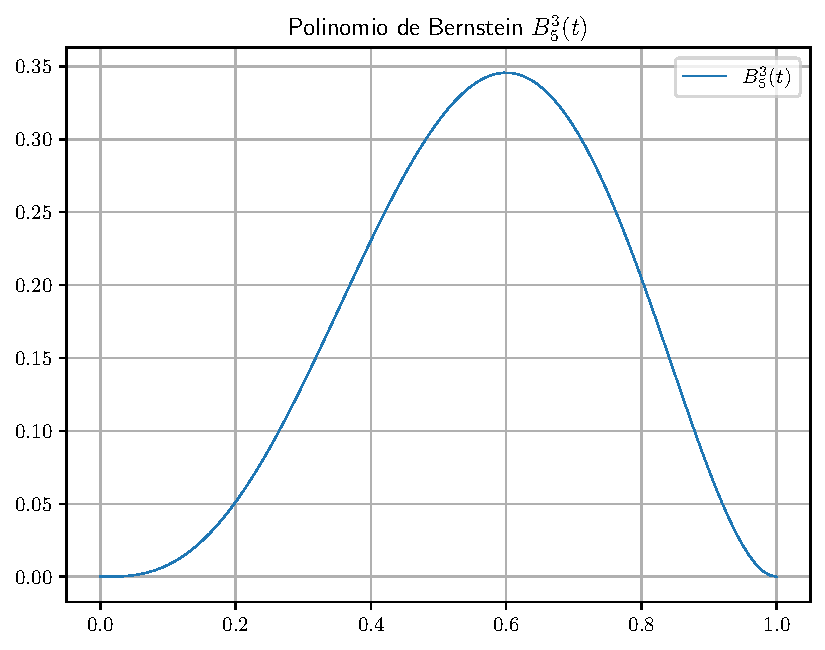
\includegraphics[width=.72\paperwidth]{p1}
        \end{figure}
    \end{solution}
\end{frame}

\begin{frame}
    \begin{solution}
        \begin{figure}[ht!]
            \centering
            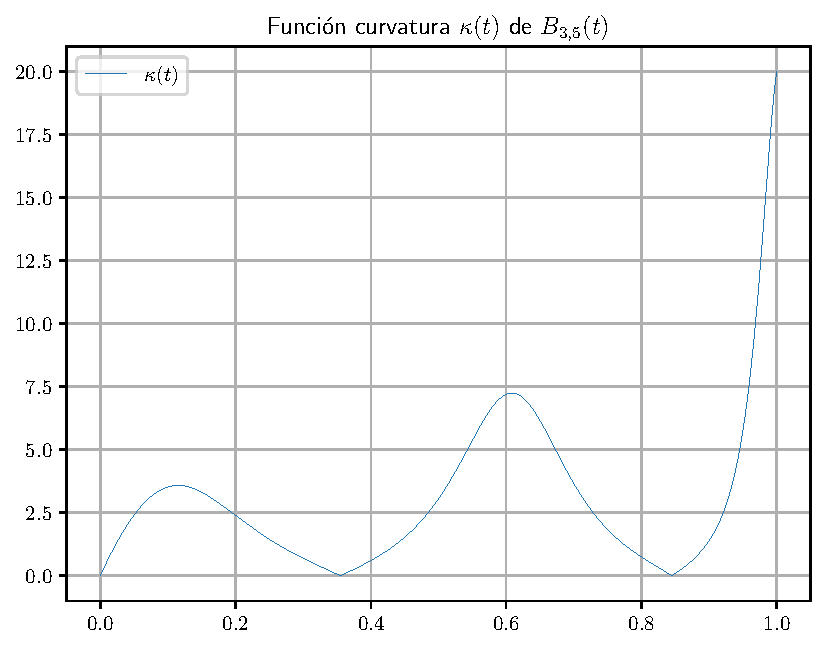
\includegraphics[width=.72\paperwidth]{p1_curvature}
        \end{figure}
    \end{solution}
\end{frame}

\begin{frame}[fragile]
    Las gráficas de los polinomios de Bernstein y su curvatura fueron
    obtenidas del programa en Python.
    \begin{solution}
        \begin{columns}
            \begin{column}{0.48\textwidth}
                \inputminted[fontsize=\tiny,firstline=3,lastline=4]{python}{p1.py}

                \

                \inputminted[fontsize=\tiny,firstline=10,lastline=20]{python}{p1.py}

            \end{column}
            \begin{column}{0.48\textwidth}
                \inputminted[fontsize=\tiny,firstline=23,lastline=27]{python}{p1.py}

                \

                \inputminted[fontsize=\tiny,firstline=34,lastline=40]{python}{p1.py}
            \end{column}
        \end{columns}
    \end{solution}
\end{frame}